\documentclass[10pt,twocolumn]{article}

\usepackage[margin=0.75in]{geometry}
\usepackage{graphicx}
\usepackage{amsmath}
\usepackage{amssymb}
\usepackage{booktabs}
\usepackage{caption}
\usepackage[colorlinks=true,allcolors=blue]{hyperref}
\usepackage{enumitem}

\captionsetup{font=small,labelfont=bf}
\setlength{\parskip}{2pt}

% This document is figure-dense (12 floats over ~7 pages). LaTeX's defaults are
% conservative about how much of a page a float may occupy, which pushes floats
% to the back and strands them on a float-only page after the conclusion. Loosen
% the fractions so floats stay near the text that references them.
\renewcommand{\topfraction}{0.9}
\renewcommand{\bottomfraction}{0.8}
\renewcommand{\textfraction}{0.07}
\renewcommand{\floatpagefraction}{0.75}
\renewcommand{\dbltopfraction}{0.9}
\renewcommand{\dblfloatpagefraction}{0.75}
\setcounter{topnumber}{3}
\setcounter{bottomnumber}{2}
\setcounter{totalnumber}{4}

\title{\vspace{-1.5em}\textbf{SoundSignal: Predicting Spotify Popularity and\\
Decomposing}\vspace{-0.5em}}
\author{Milan Giliazetdinov}
\date{}

\begin{document}
\maketitle

\begin{abstract}
\noindent
Predicting a song's Spotify popularity is only half of a useful answer. A single
blended score cannot tell a musician whether a track scored well because the
artist is already famous, because the genre is commercially favoured, or because
of the recording itself. This project trains a gradient-boosted model on 66{,}808
cleaned tracks and then \emph{decomposes} its prediction into four additive
terms: a typical-track baseline, artist fame, genre, and the recording's own
contribution. Along the way two instructive failures were documented: a
leave-one-out artist-fame feature that silently leaked the target
($\rho = 0.85$ with popularity), and an evaluation setup in which forgetting to
remove genre inflated the apparent audio signal roughly $3.5\times$
($0.128 \rightarrow 0.460$ Spearman). The final composed model reaches
$R^2 = 0.6206$ and Spearman $0.7917$, and the honest measured finding is that
the contribution attributable to audio alone is small once fame and genre are
accounted for.
\end{abstract}

\section{Introduction}

Spotify assigns every track a \emph{popularity} score from 0 to 100. Predicting
it is a standard regression problem, but a prediction alone is commercially
uninteresting to the person who made the song: it does not separate what the
artist's existing audience contributed from what the record contributed.

This project therefore has two goals. The first is conventional --- try fit the best
model possible. The second is the actual product: split the
predicted number into interpretable, additive parts, so that
\begin{equation}
\hat{y} \;=\; b \;+\; \Delta_{\text{fame}} \;+\; \Delta_{\text{genre}} \;+\; \Delta_{\text{audio}}
\label{eq:decomp}
\end{equation}
holds exactly, and each term can be shown to a user with a defensible meaning.

Two models are trained. A \textbf{research model} uses Spotify's own engineered
audio features (danceability, valence, energy, and so on) and exists to answer
the modelling question as well as possible. A \textbf{production model} uses
\texttt{librosa} descriptors computed directly from an uploaded mp3, because
Spotify deprecated public access to its audio-features endpoint and those
features are simply unavailable for a user's own file.

\section{Dataset and Preprocessing}

\subsection{The raw data}

The starting corpus contains 114{,}000 Spotify tracks with audio features,
genre labels, and popularity (Figure~\ref{fig:raw_desc},
Figure~\ref{fig:raw_dist}). It is not usable as delivered. A large share of rows
are duplicate copies of original songs that appeared in user playlists under
different track identifiers. These duplicates carry near-zero popularity while
being, musically, the same recording as a well-known track. Left in place they
teach the model that famous songs are unpopular.

\subsection{Building an artist-fame signal}

Removing those rows requires knowing whether the \emph{artist} is significant,
and Spotify's dataset ships no artist-popularity field. We therefore constructed
one by target encoding: for track $i$ by artist $a$, average the popularity of
that artist's \emph{other} tracks,
\begin{equation}
\texttt{artist\_fame\_loo}_i \;=\; \frac{1}{|A_i| - 1}\sum_{j \in A_i,\, j \neq i} y_j ,
\label{eq:loo}
\end{equation}
where $A_i$ is the set of tracks by artist $a$. The leave-one-out construction
excludes $y_i$ itself, which is what prevents a song's own popularity from
flowing directly into its own feature. This worked well for \emph{cleaning}: a
track whose artist averages a high popularity but which itself sits at zero is
almost certainly a playlist duplicate, and can be dropped. Cleaning reduced
114{,}000 rows to \textbf{66{,}808}.

It did not work as a \emph{feature}. Equation~\ref{eq:loo} is still built out of
the target variable, and it shows: \texttt{artist\_fame\_loo} correlates with
popularity at $\rho = 0.85$ (Figure~\ref{fig:corr}). A model given it reports
strong results that are largely the target predicting itself. It is also
uncomputable at serving time, since a newly uploaded song has no catalogue of
sibling tracks to average.

It was decided to replaced it with an external signal: total listener counts per artist pulled
from the Last.fm API. This feature has an honest weakness --- a large listener
count is not the same thing as fame, since it accumulates over time and rewards
longevity as much as current standing --- but no better public alternative was
available, and critically it correlates with popularity at only $\rho = 0.42$,
i.e.\ it carries information without being a proxy for the answer.

\subsection{Scaling}

Both \texttt{duration\_ms} and \texttt{artists\_listeners} are strongly
right-skewed and live on scales orders of magnitude larger than the $[0,1]$
audio features. We apply $x \mapsto \log(x)$ to both, which compresses the tail
onto a comparable range (Figure~\ref{fig:clean_desc}). This matters most for the
linear models, where a feature's scale directly affects its coefficient and any
regularisation penalty applied to it.

\begin{figure*}[t]
\centering
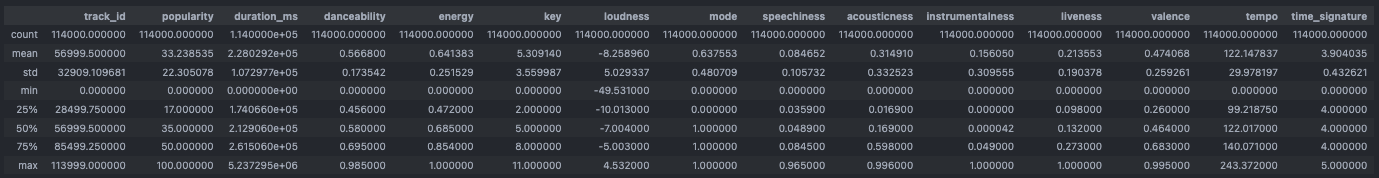
\includegraphics[width=\textwidth]{figures/raw_data_description.png}
\caption{Descriptive statistics of the raw 114{,}000-track dataset. Popularity
averages 33.2 with a first quartile of 17, pulled down by the playlist
duplicates; \texttt{duration\_ms} spans four orders of magnitude, motivating the
log transform.}
\label{fig:raw_desc}
\end{figure*}

\begin{figure}[t]
\centering
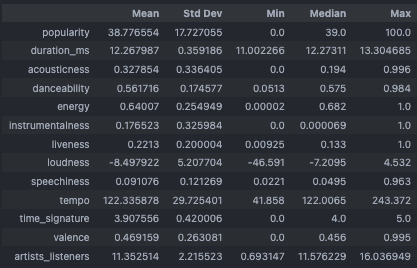
\includegraphics[width=\columnwidth]{figures/cleaned_data_description.png}
\caption{Descriptive statistics after cleaning (66{,}808 tracks). Note
\texttt{duration\_ms} and \texttt{artists\_listeners} are log-transformed.}
\label{fig:clean_desc}
\end{figure}

\section{Exploratory Data Analysis}

Figures~\ref{fig:raw_dist} and~\ref{fig:clean_dist} show feature distributions
before and after cleaning. Most audio features are close to normally
distributed; \texttt{speechiness}, \texttt{instrumentalness}, \texttt{liveness}
and \texttt{acousticness} are heavily concentrated near zero, which is expected
given that most commercially released tracks are studio recordings with sung
vocals.

The Spearman correlation matrix (Figure~\ref{fig:corr}) drives the modelling
strategy. Against popularity, the two strongest relationships by a wide margin
are \texttt{artists\_listeners} ($0.42$) and genre; every individual audio
feature sits near zero, the largest being \texttt{danceability} at $0.11$ and
\texttt{instrumentalness} at $-0.19$. Among features themselves the structure is
musically sensible: energy and loudness move together ($0.75$), energy and
acousticness oppose one another ($-0.71$), and danceability tracks valence
($0.47$).

\begin{figure*}[t]
\centering
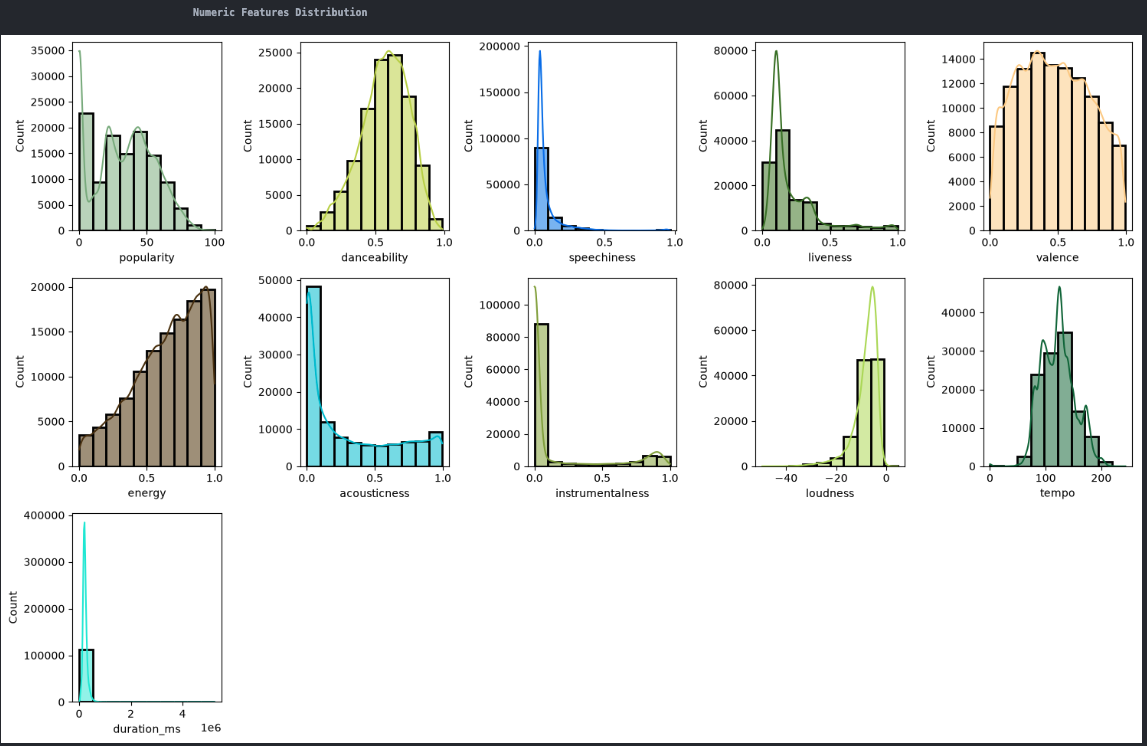
\includegraphics[width=0.78\textwidth]{figures/raw_distributions.png}
\caption{Numeric feature distributions in the raw 114{,}000-track dataset.
Popularity has a large spike at zero --- the playlist duplicates.}
\label{fig:raw_dist}
\end{figure*}

\begin{figure*}[t]
\centering
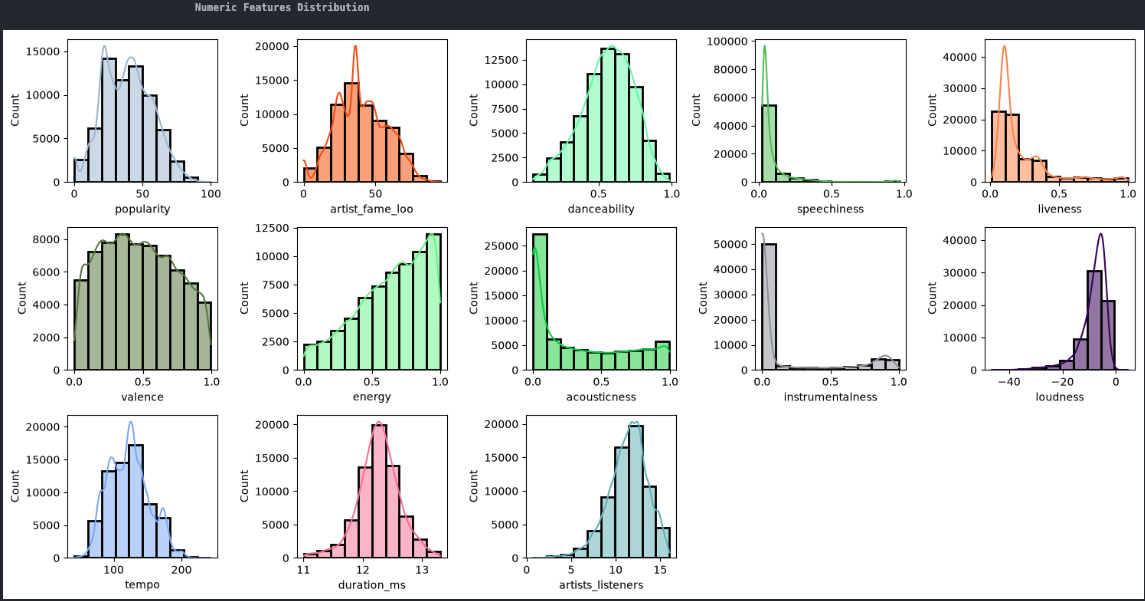
\includegraphics[width=0.78\textwidth]{figures/cleaned_distributions.png}
\caption{Numeric feature distributions after cleaning. The zero-popularity spike
is gone and popularity is approximately normal.}
\label{fig:clean_dist}
\end{figure*}

\begin{figure*}[t]
\centering
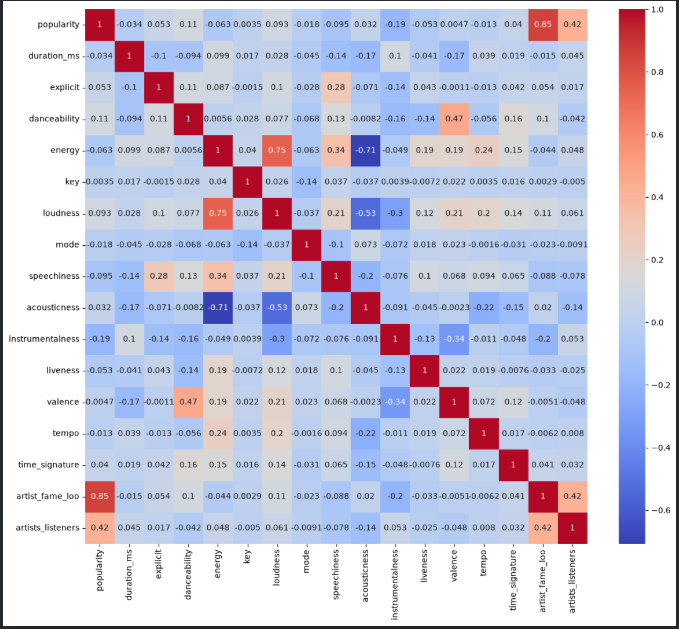
\includegraphics[width=0.58\textwidth]{figures/spearman_correlation.png}
\caption{Spearman correlation matrix. \texttt{artist\_fame\_loo} correlates
$0.85$ with popularity --- the target leak that forced its removal --- against
$0.42$ for the external \texttt{artists\_listeners} replacement.}
\label{fig:corr}
\end{figure*}

\section{Model Selection}

It was decided to try several models for both baseline estimation and understanding of structure of data.

\subsection{Ordinary least squares}

OLS fits a linear map $\hat{y} = X\beta$ by minimising squared error,
\begin{equation}
\hat{\beta} \;=\; \arg\min_{\beta} \lVert y - X\beta \rVert_2^2
\;=\; (X^\top X)^{-1} X^\top y ,
\end{equation}
and serves as the baseline. Genre is nominal and must be one-hot encoded, which
expands $X$ by 114 columns. Results are in Figure~\ref{fig:ols}: test
$R^2 = 0.5983$, MAE $8.269$, RMSE $11.310$. Train and test scores are nearly
identical ($R^2 = 0.6009$ vs $0.5983$).

\subsection{Lasso}

With genre one-hot encoded, most of the design matrix is sparse indicator
columns, many of which are likely uninformative. Lasso adds an $L_1$ penalty,
\begin{equation}
\hat{\beta} \;=\; \arg\min_{\beta} \frac{1}{2n}\lVert y - X\beta \rVert_2^2
\;+\; \alpha \lVert \beta \rVert_1 ,
\end{equation}
whose non-differentiable corner at the origin drives coefficients to \emph{exactly}
zero rather than merely shrinking them. It therefore performs implicit feature
selection, which is the reason to prefer it here over ridge regression. Under
nested cross-validation (Figure~\ref{fig:lasso}) it reaches $R^2 = 0.5984$,
MAE $8.277$, RMSE $11.233$.

\subsection{Diagnosis: high bias, not high variance}

Lasso performs essentially identically to OLS ($0.5984$ vs $0.5983$), and OLS
train and test scores barely differ. Regularisation changing nothing means
variance is not the limiting factor. Combined with high absolute error, this is
the signal of \textbf{high bias}. Hence the hypothesis class is: model is too simple to for the data, and hence a more complex model should be utilized.

\subsection{Multilayer perceptron}

A neural network with one hidden layer computes
\begin{equation}
h = \sigma(W_1 x + b_1), \qquad \hat{y} = W_2 h + b_2 ,
\end{equation}
where the non-linear activation $\sigma$ allows curved decision surfaces that no
linear model can express. It improves notalby (Figure~\ref{fig:mlp}): test
$R^2 = 0.6494$, MAE $7.285$, RMSE $10.540$. The gap between train $R^2 = 0.7284$
and test $0.6494$ indicates mild overfitting, but the the hypothesis is proven:
\textbf{the data has non-linear relationship}. Given that \texttt{artists\_listeners} is the
dominant numeric predictor, this implies the fame-to-popularity relationship is
curved. This makes a perfect sense, since the difference between
10{,}000 and 1{,}000{,}010 listeners matters far more than between 5M and 6M.

That conclusion is what motivates tree ensembles, which capture non-linearity
and interactions natively and handle the mixed continuous/categorical feature
space without one-hot encoding.

\subsection{Tree ensembles}


Totally the performance of four ensembles (Figure~\ref{fig:trees}) was evaluated. \textbf{Random forests}
average $B$ decorrelated trees grown on bootstrap samples,
\begin{equation}
\hat{y} = \frac{1}{B}\sum_{b=1}^{B} T_b(x) ,
\end{equation}
reducing variance through averaging. \textbf{Extremely randomised trees} go
further and draw split thresholds at random, trading a little extra bias for
another variance reduction. Both are \emph{bagging} methods: trees are grown
independently and in parallel.

\textbf{Gradient boosting} is structurally different. It fits trees in sequence,
each one correcting its predecessors' errors:
\begin{equation}
F_m(x) \;=\; F_{m-1}(x) \;+\; \nu\, h_m(x) ,
\end{equation}
where $h_m$ is fitted to approximate the negative gradient of the loss,
$-\partial \mathcal{L}(y, F_{m-1}) / \partial F_{m-1}$, and $\nu$ is the learning
rate. Because each tree targets the residual error left by the ensemble so far,
boosting builds far more expressive functions than an average of independent
trees.

The results follow that ordering: RandomForest is worst
($R^2_{\text{holdout}} = 0.5865$), the two boosting variants and ExtraTrees
cluster around $0.64$--$0.65$, and \textbf{LightGBM} --- a gradient booster using
leaf-wise tree growth and histogram-binned features --- performed best overall,
reaching $R^2 = 0.7067$, MAE $6.537$ and Spearman $0.8411$
(Figure~\ref{fig:lgbm}).

Its feature importances make the central finding of the whole project explicit:
\texttt{track\_genre} (1863) and \texttt{artists\_listeners} (1614) dominate,
while every audio feature lands between 471 and 618. The conclusion here is that the context rather than sound,
explains most of popularity.

\begin{figure}[t]
\centering
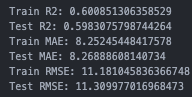
\includegraphics[width=0.92\columnwidth]{figures/ols_results.png}
\caption{OLS on Spotify features. Train and test are nearly identical.}
\label{fig:ols}
\end{figure}

\begin{figure}[t]
\centering
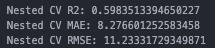
\includegraphics[width=0.92\columnwidth]{figures/lasso_results.png}
\caption{Lasso under nested cross-validation --- statistically indistinguishable
from OLS, indicating bias rather than variance is the bottleneck.}
\label{fig:lasso}
\end{figure}

\begin{figure}[t]
\centering
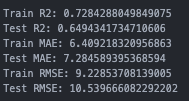
\includegraphics[width=0.92\columnwidth]{figures/mlp_results.png}
\caption{MLP results. The jump over the linear models is evidence of a
non-linear fame-to-popularity relationship.}
\label{fig:mlp}
\end{figure}

\begin{figure}[tb]
\centering
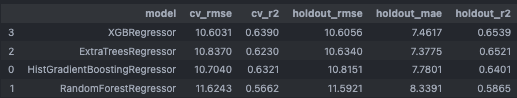
\includegraphics[width=\columnwidth]{figures/tree_models_results.png}
\caption{Tree ensemble comparison under cross-validation and on a holdout set.
The boosting methods and ExtraTrees cluster around $R^2 \approx 0.64$--$0.65$;
the plain random forest trails at $0.5865$.}
\label{fig:trees}
\end{figure}

\begin{figure}[t]
\centering
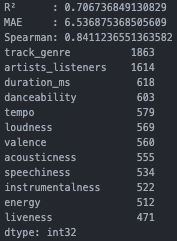
\includegraphics[width=0.85\columnwidth]{figures/lgbm_results.png}
\caption{LightGBM: best overall, and its feature importances show genre and
artist listeners dominating every audio feature.}
\label{fig:lgbm}
\end{figure}

\section{From Spotify Features to librosa}

The research model above cannot be deployed. Spotify deprecated public access to
its audio-features endpoint, so when a user uploads an mp3 there is no way to
obtain \texttt{danceability} or \texttt{valence} for it. Two options existed.

\textbf{Option A} was to estimate Spotify's features from signal-level
descriptors --- train a model per feature, then feed the estimates into the
existing pipeline. Its appeal is interpretability, since the final explanation
could keep using familiar names. It was decided to reject this idea. Spotify's features are
themselves the output of proprietary models almost certainly more sophisticated
than a linear or tree regressor; approximating them with a simpler model
degrades the signal, and that degraded estimate is then consumed by a second
model whose own error compounds it. The layer cannot add information that the
signal-level descriptors did not already carry.

\textbf{Option B}, which was adopted, is to retrain the audio model directly on
\texttt{librosa} descriptors extracted from the waveform: tempo, onset rate, RMS
energy and dynamic range, spectral centroid, bandwidth, rolloff, flatness and
contrast, zero-crossing rate, MFCCs, and chroma statistics.

The empirical result vindicates the choice. On identical rows, the librosa audio
model reaches a residual Spearman of \textbf{0.128} against \textbf{0.125} for
Spotify's own engineered features, with a shuffled-feature control at $0.008$
(Figure~\ref{fig:audio_genre}, left). Speaking librosa costs essentially
nothing.

\section{The Serving Pipeline}

\subsection{Why Spearman}

Spearman's rank correlation was used
\begin{equation}
\rho \;=\; \operatorname{corr}\!\big(\operatorname{rank}(y), \operatorname{rank}(\hat{y})\big),
\end{equation}
as a headline metric alongside MAE, RMSE and
$R^2 = 1 - \sum(y_i-\hat y_i)^2 / \sum(y_i-\bar y)^2$. The reason is that
Spotify's popularity value is an abstract, recency-weighted index whose absolute
magnitude is hard to interpret, whereas \emph{ordering} songs correctly is
directly meaningful and is what the product actually presents.

\subsection{The key insight: genre is audio}

Audio features alone yield only about $0.13$ Spearman on the residual, and the
LightGBM importances put genre and fame far ahead. At first it might seem that the audio does not matter -- but this is wrong assumption.

Genre \emph{is} audio. A genre label is essentially a name attached to a region
of audio-feature space: acousticness separates classical, energy and distortion
separate metal, speechiness separates rap. When genre is included as a feature it
absorbs that shared information first, leaving audio only whatever is left over.

This is measurable. Removing genre from the context model, so that only fame is
residualised out, raises the audio model's Spearman from $0.128$ to
\textbf{0.460} for librosa and from $0.125$ to $0.429$ for the Spotify features
--- roughly a $3.5\times$ inflation (Figure~\ref{fig:audio_genre}, right). The
apparent gain is not new signal; it is the audio model re-identifying genre.

This cuts both ways, and both directions matter. It proves audio genuinely
carries popularity-relevant information. It also proves that an evaluation which
forgets to remove genre will dramatically overstate the audio model's ability to
judge a \emph{song}, and that comparing a pop track's audio against a classical
track's is not a fair comparison. The decomposition below is therefore
constructed per genre.

\begin{figure*}[t]
\centering
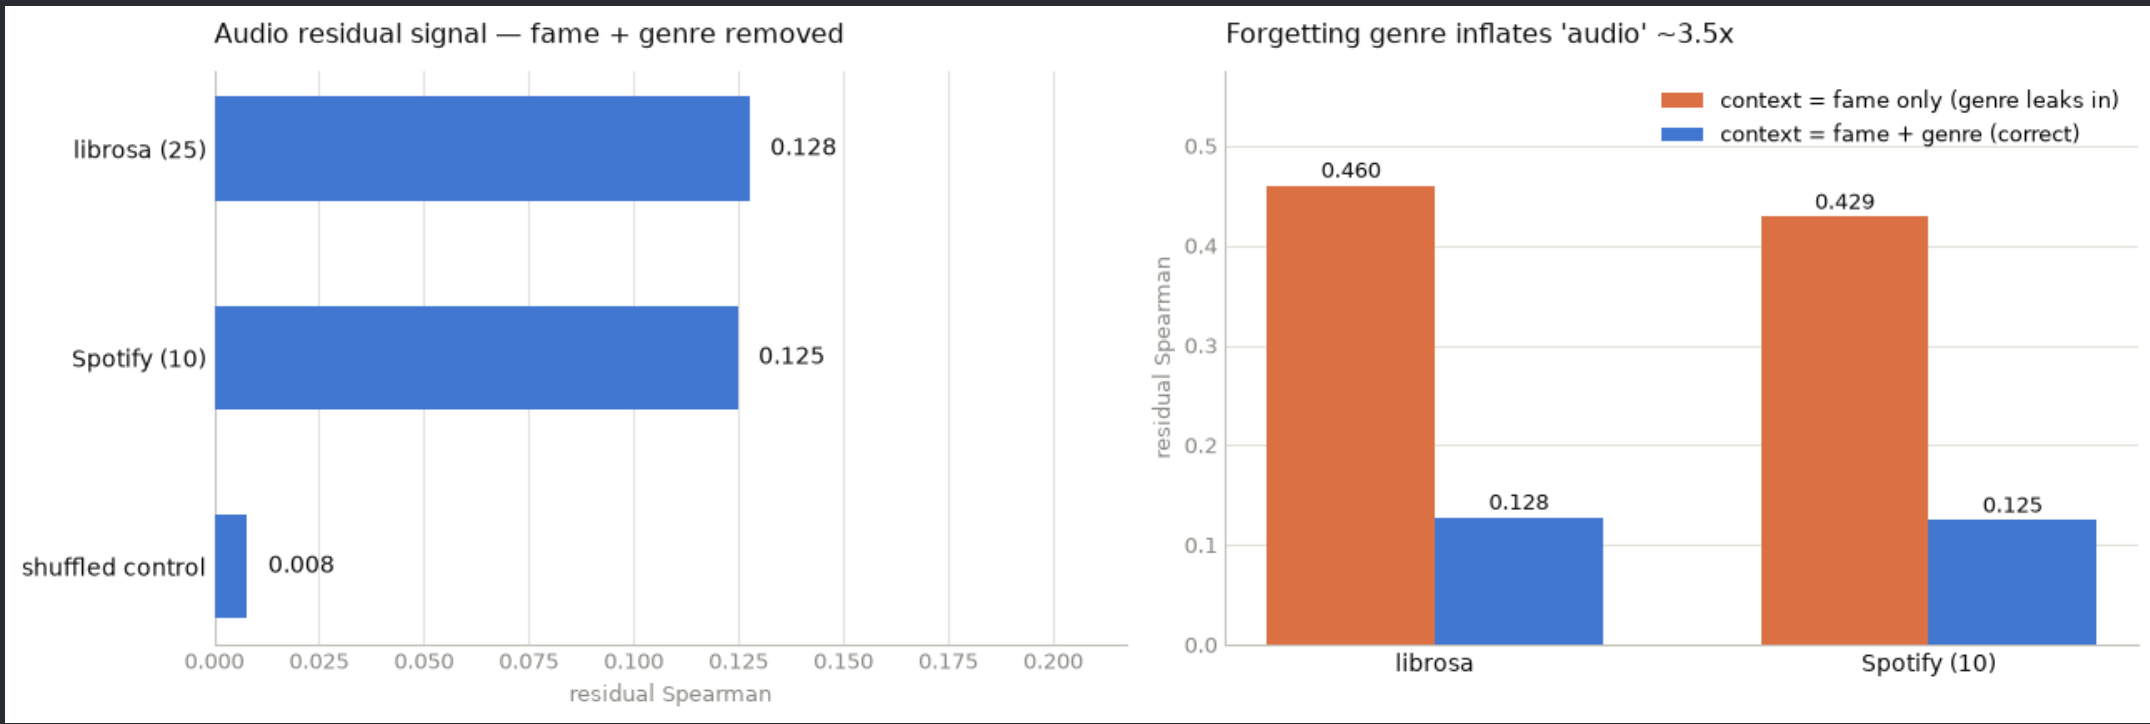
\includegraphics[width=0.94\textwidth]{figures/audio_genre_comparison.png}
\caption{Left: with fame \emph{and} genre removed, librosa (0.128) and Spotify's
engineered features (0.125) are near-identical, both far above the shuffled
control (0.008). Right: residualising on fame alone leaves genre in the target
and inflates the apparent audio signal roughly $3.5\times$.}
\label{fig:audio_genre}
\end{figure*}

\subsection{The four-term decomposition}

Let $L$ denote an artist's listener count, $g$ a genre, $G$ the set of training
genres, $f_c$ the context model (fame and genre), $f_a$ the audio model, and $z$
a track's librosa features. Define the \emph{marginal} context prediction at
fame level $L$, with genre integrated out:
\begin{equation}
m(L) \;=\; \frac{1}{|G|}\sum_{g \in G} f_c(L, g).
\end{equation}

\paragraph{Typical track.} The baseline is the marginal prediction at the median
listener count $\tilde{L}$, i.e.\ a median-fame artist in an average genre:
\begin{equation}
b \;=\; m(\tilde{L}).
\end{equation}

\paragraph{Artist fame.} How much this artist's audience moves the score away
from that baseline, with genre still averaged out so the term isolates fame:
\begin{equation}
\Delta_{\text{fame}} \;=\; m(L) - b.
\end{equation}

\paragraph{Genre.} How much \emph{this} genre is worth at \emph{this} artist's
level of fame, plus a correction $o_g$ defined below:
\begin{equation}
\Delta_{\text{genre}} \;=\; f_c(L, g) - m(L) + o_g .
\end{equation}

\paragraph{Audio.} The audio model is trained not on popularity but on the
\emph{residual} --- what fame and genre could not explain:
\begin{equation}
r_i \;=\; y_i - \hat{y}^{(-k)}_{c,i},
\end{equation}
where $\hat{y}^{(-k)}_{c,i}$ is an out-of-fold context prediction. The
recording's contribution is then the audio model's output minus the same
per-genre offset:
\begin{equation}
\Delta_{\text{audio}} \;=\; f_a(z) - o_g .
\end{equation}

\paragraph{The per-genre offset.} Even after residualising, the audio model's
output retains a mild genre bias, because the context model's removal of genre is
imperfect. The offset is the mean out-of-fold audio prediction within genre $g$,
\begin{equation}
o_g \;=\; \frac{1}{|S_g|}\sum_{i \in S_g} \hat{r}^{(-k)}_i ,
\end{equation}
over the set $S_g$ of calibration tracks in that genre. Subtracting it from the
audio term and adding it to the genre term moves that systematic component to
where it belongs. Since the same quantity is subtracted from one term and added
to another, the total in Equation~\ref{eq:decomp} is unchanged --- the
decomposition still sums exactly to the prediction, but the audio term now
measures deviation \emph{within} a genre rather than membership \emph{of} one.

\subsection{Out-of-fold estimation}

Both the residual target and the offset are computed out-of-fold: the data is
partitioned into $k$ folds, and each sample is scored by a model trained without
it. An in-sample prediction is partly memorised, which biases residuals toward
zero and would corrupt the audio model's target. The context model uses a
10-fold \texttt{GroupKFold} split grouped by primary artist, so no artist appears
in both training and validation --- otherwise the model can learn
artist-specific residuals, reintroducing exactly the fame effect the
residualisation was designed to remove.

\subsection{Calibration}

A raw contribution of $+2.1$ points does not tell a user whether $+2.1$ is good.
We therefore calibrate the audio term into a within-genre percentile:

\begin{enumerate}[leftmargin=*,topsep=2pt,itemsep=1pt]
  \item Predict popularity from context (fame and genre).
  \item Compute residuals $r_i = y_i - \hat{y}^{(-k)}_{c,i}$.
  \item Train the audio model on those residuals.
  \item Produce an out-of-fold audio prediction for every calibration track.
  \item Build a 101-point percentile grid per genre from those predictions.
  \item Compute the per-genre offset $o_g$.
\end{enumerate}

The grid is built from \emph{predictions} rather than true residuals because a
model with modest explanatory power correctly hedges toward the mean: its outputs
span a far narrower range than the target does. Ranking predictions against the
true-residual spread would compress every song into the middle of the scale.
Genres with too few calibration tracks fall back to the global grid.

\subsection{Composed performance}

Figure~\ref{fig:overall} gives the final ablation. Adding audio to fame and
genre improves every metric --- MAE $7.708 \rightarrow 7.694$, RMSE
$11.026 \rightarrow 11.013$, $R^2$ $0.6198 \rightarrow 0.6206$, Spearman
$0.7880 \rightarrow 0.7917$. The improvement is real and consistent, and it is
small. That is the honest result: once an artist's reach and a track's genre are
known, the recording itself adjusts the expected popularity by a few points.

\begin{figure}[t]
\centering
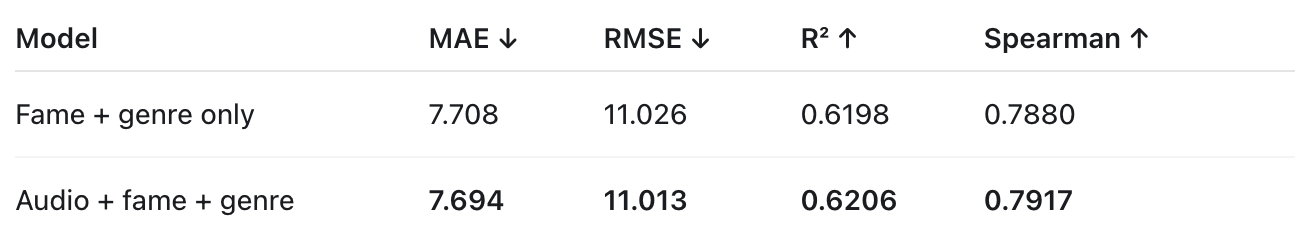
\includegraphics[width=\columnwidth]{figures/overall_performance.png}
\caption{Composed pipeline. Audio improves every metric over fame and genre
alone, by a small and consistent margin.}
\label{fig:overall}
\end{figure}

\section{Explanation Layer}

The decomposition is only useful if a musician can read it, and terms like
``MFCC 7'' or ``spectral flatness'' are not readable. The final stage converts
the numbers into plain English.

Attribution uses SHAP values, which distribute a prediction across its features
according to the Shapley value from cooperative game theory:
\begin{equation}
\phi_j = \!\!\sum_{S \subseteq F \setminus \{j\}}\!\!
\frac{|S|!\,(|F|-|S|-1)!}{|F|!}\big[f(S \cup \{j\}) - f(S)\big].
\end{equation}
The property that makes this usable is additivity:
\begin{equation}
f(x) \;=\; \phi_0 + \sum_{j} \phi_j ,
\end{equation}
so the parts provably sum to the whole. Because SHAP values are additive, related
descriptors can be summed into groups without breaking that guarantee --- the 58
librosa descriptors are folded into 12 human-readable concepts such as
brightness, note density, dynamic range and overall timbre. This is also the only
honest way to discuss MFCCs, since no individual coefficient has a meaning worth
reporting.

Those grouped values are serialised to JSON and passed to a locally hosted large
language model, together with a predefined glossary explaining what each concept
means. The model's role is strictly translation: it verbalises numbers that were
already computed, and it neither predicts nor attributes anything itself.

\section{Conclusion and Limitations}

The composed model reaches $R^2 = 0.6206$ and Spearman $0.7917$, and decomposes
every prediction into four terms that sum to it exactly.

Three limitations deserve statement. First, the target is noisy: Spotify's
popularity index is a recency-weighted black box, so small differences between
models should not be over-read. Second, \texttt{artists\_listeners} measures
cumulative reach rather than current fame, and rewards longevity. Third, and most
importantly, the audio contribution is genuinely small once fame and genre are
removed --- and the $0.128 \rightarrow 0.460$ result shows precisely how easy it
would be to report a much more flattering number by residualising on fame alone.
The project's central methodological claim is that resisting that temptation is
what makes the remaining number trustworthy.

\end{document}
